% Created 2022-01-27 Thu 12:16
% Intended LaTeX compiler: pdflatex
\documentclass[11pt]{article}
\usepackage[utf8]{inputenc}
\usepackage[T1]{fontenc}
\usepackage{graphicx}
\usepackage{longtable}
\usepackage{wrapfig}
\usepackage{rotating}
\usepackage[normalem]{ulem}
\usepackage{amsmath}
\usepackage{amssymb}
\usepackage{capt-of}
\usepackage{hyperref}
\usepackage{color}
\usepackage{listings}
\usepackage{color}
\usepackage{listings}
\author{Maikol Solís}
\date{\textit{[2022-01-27 Thu 11:10]}}
\title{Mi primera nota}
\hypersetup{
 pdfauthor={Maikol Solís},
 pdftitle={Mi primera nota},
 pdfkeywords={},
 pdfsubject={},
 pdfcreator={Emacs 27.2 (Org mode 9.6)}, 
 pdflang={English}}
\usepackage{biblatex}

\begin{document}

\maketitle
\tableofcontents

Esta es mi primera nota

Otra modificación

Nueva modificación.


\begin{center}
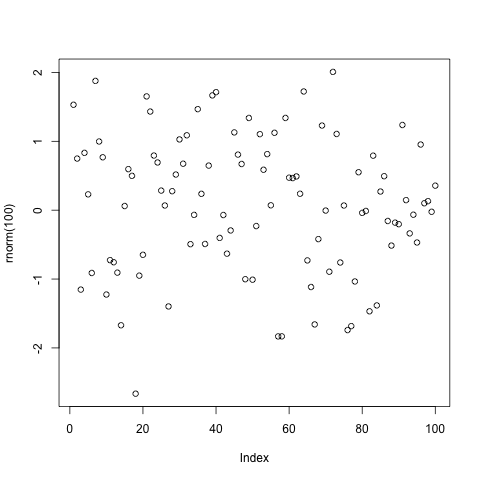
\includegraphics[width=.9\linewidth]{20220127T111026-figure-1-grafico_de_normales.png}
\end{center}
\end{document}